\section{Uniform Random Numbers}
Let $U$ be a uniform random variable between 0 and 1.
\begin{enumerate}
\item Generate $10^6$ samples of $U$ using a C program and save into a file called uni.dat .
\label{prob:uni_gen}
\\
\solution Download the following files and execute the  C program.
\begin{lstlisting}
	chapter2/codes/exrand.c
    chapter2/codes/coeffs.h
\end{lstlisting}

%
\item
Load the uni.dat file into python and plot the empirical CDF of $U$ using the samples in uni.dat. The CDF is defined as
\begin{align}
F_{U}(x) = \pr{U \le x}
\end{align}

\begin{lstlisting}
chapter2/codes/cdf_plot.py	
\end{lstlisting}
\begin{figure}[H]
\centering
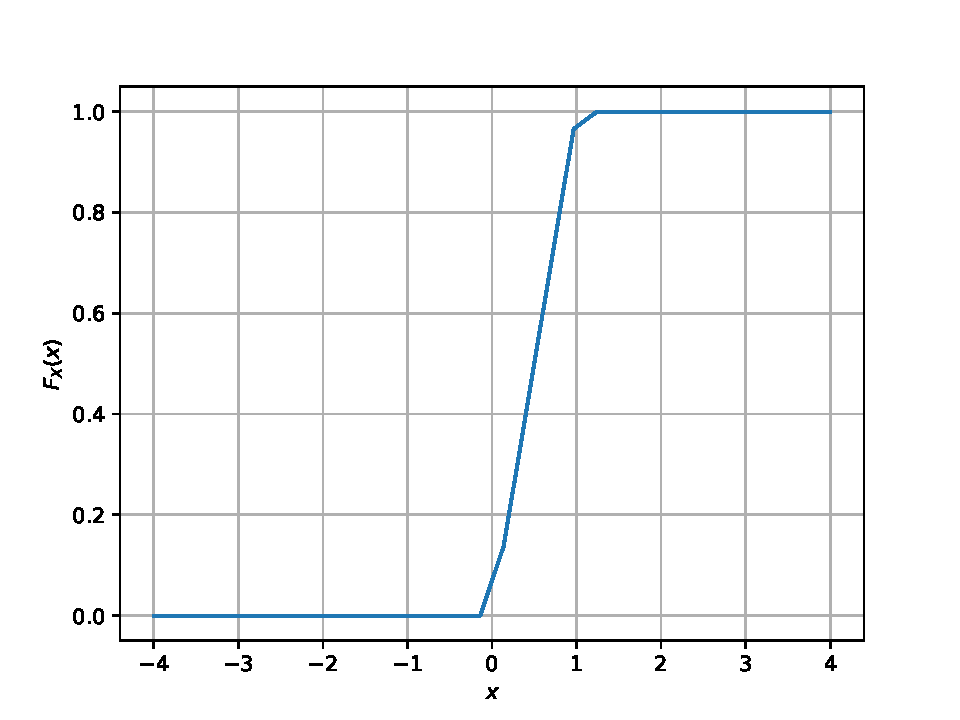
\includegraphics[scale=0.8]{chapter2/figs/uni_cdf.pdf}
\caption{The CDF of $U$}
\label{fig:uni_cdf}
\end{figure}
\item
Find a  theoretical expression for $F_{U}(x)$.\\
\solution
%\begin{align} 
%F_{U}(x) = \int_{-\infty}^{x} f_{U}(x)\,dx
%\label{eq:pdf_to_cdf}
%\end{align}
%For the uniform random variable $U$, $f_{U}(x)$ is given by  
%\begin{align}
%	f_U(x) &= 
%	\begin{cases}
%	1 &  0 \le x \le  1
%	\\
%	0 & elsewhere
%	\\
%	\end{cases}
%	\label{eq:uni_pdf}
%\end{align}
%Substituting \eqref{eq:uni_pdf} in \eqref{eq:pdf_to_cdf}, $F_U(x)$ is found to be
\begin{align}
	F_U(x) &= 
	\begin{cases}
	0 & x < 0
	\\	
	x & 0 \le x \le  1
	\\
	1 & x > 0
	\\
	\end{cases}
	\label{eq:uni_cdf}
\end{align}

\item
\label{prob:print_uni}
The mean of $U$ is defined as
%
\begin{equation}
E\sbrak{U} = \frac{1}{N}\sum_{i=1}^{N}U_i
\end{equation}
%
and its variance as
%
\begin{equation}
\text{var}\sbrak{U} = E\sbrak{U- E\sbrak{U}}^2 
\end{equation}

Write a C program to  find the mean and variance of $U$.\\
\solution The code below is the function for calculating mean
\begin{lstlisting}
	double mean(char *str)
{
int i=0,c;
FILE *fp;
double x, temp=0.0;

fp = fopen(str,"r");
//get numbers from file
while(fscanf(fp,"%lf",&x)!=EOF)
{
//Count numbers in file
i=i+1;
//Add all numbers in file
temp = temp+x*x;
}
fclose(fp);
temp = temp/(i-1);
return temp;

}
\end{lstlisting}
Function for calculating the mean
\begin{lstlisting}
double variance(char *str)
{
int i=0,c;
FILE *fp;
double x, sum_square=0.0, temp=0.0, var;

fp = fopen(str,"r");
//get numbers from file
while(fscanf(fp,"%lf",&x)!=EOF)
{
//Count numbers in file
i=i+1;
//Add all numbers in file
temp += x;
sum_square += (x*x);
}
fclose(fp);
var = (sum_square - temp*temp/(i-1))/(i-2);
return var;

}
\end{lstlisting}
The following code prints the mean and variance of $U$
\begin{lstlisting}
	chapter2/codes/mv.c
\end{lstlisting}
The output of the program is
\begin{lstlisting}
Uniform stats:
Mean: 0.500007
Variance: 0.083301
\end{lstlisting}

\item Verify your result theoretically given that
%
\begin{equation}
E\sbrak{U^k} = \int_{-\infty}^{\infty}x^kdF_{U}(x)
\end{equation}\\
\solution For a random variable $X$, the mean $\mu_X$ is given by
\begin{align}
	\label{eq:mean_exp}
	\mu_X &= E\sbrak{X} = \int_{-\infty}^{\infty}xdF_{U}(x) \\
	\label{eq:var_exp}
	\sigma_X^2 &= E\sbrak{X^2} - \mu_X^2 = \int_{-\infty}^{\infty}x^2dF_{U}(x) - \mu_X^2
\end{align} 
Variance $\sigma_X^2$ is given by
 
Substituting the CDF of $U$ from (2.1.3.3) in (2.1.5.2) and (2.1.5.3), we get \\
 \begin{align}
	\label{eq:mean_uni}
	\textbf{Mean} & =\mu_U & \\
 \mathrm{E}[X]=\int_a^b x \cdot \frac{1}{b-a} d x
 \\ Here \  a=0,b=1
 \\ \mu= \mathrm{E}[X]= \frac{1}{2} = 0.5	\\
	\label{eq:var_uni}
	\mathrm{E}[X^2]=\int_a^b x^2 \cdot \frac{1}{b-a} d x=\frac{b^3-a^3}{3} \cdot \frac{1}{b-a} \\
 \text{Variance} \\
 \sigma^2=E\left(X^2\right)-[E(X)]^2
 =\frac{(a-b)^2}{12}\\
  \sigma^2 = \frac{1}{12} & = 0.08
\end{align} 
Hence, the output values of program and theory are same.
\end{enumerate}
\section{Central Limit Theorem}
\begin{enumerate}
\item
Generate $10^6$ samples of the random variable
%
\begin{equation}
X = \sum_{i=1}^{12}U_i -6
\end{equation}
%
using a C program, where $U_i, i = 1,2,\dots, 12$ are  a set of independent uniform random variables between 0 and 1
and save in a file called gau.dat\\
\solution Use the following code and it will generate gau.dat file with the required Random variables the  C program.
\begin{lstlisting}
	chapter2/codes/rv.c
\end{lstlisting}
%
\item
Load gau.dat in python and plot the empirical CDF of $X$ using the samples in gau.dat. What properties does a CDF have?
\\
\begin{figure}[h!]
\centering
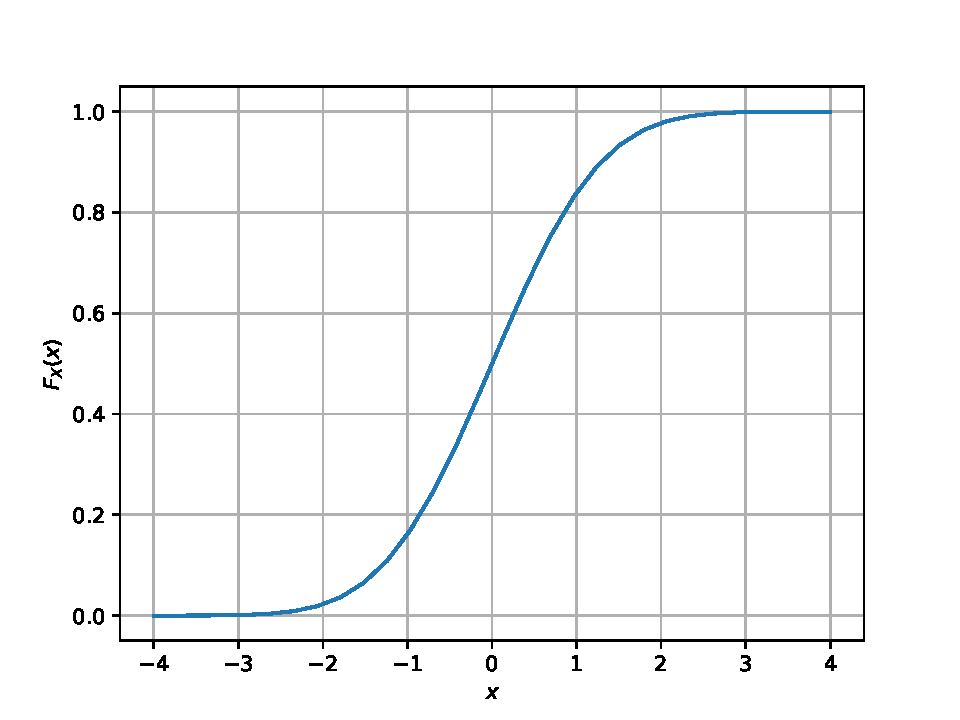
\includegraphics[scale=0.8]{chapter2/figs/gauss_cdf.pdf}
\caption{The CDF of $X$}
\label{fig:gauss_cdf}
\end{figure}
Let $X$ be a random variable (either continuous or discrete), then the CDF
of $X$ has the following properties \\
The CDF is a non-decreasing \\
The maximum of the CDF is when
\begin{eqnarray}
x = \infty: F_X(\infty) = 1
\end{eqnarray}
The minimum of the CDF is when
\begin{eqnarray}
x = -\infty: F_X(-\infty) = 0	
\end{eqnarray} 
If the CDF $F_X$ is continuous at any
$a \le x \le b$, then
\begin{eqnarray}
\Pr \lsbrak a \le X \le \rsbrak b  = F_X (b) - F_X (a)
\end{eqnarray}
For any random variable X (discrete or continuous), $P[X = b]$ is
\begin{eqnarray}
\Pr \lsbrak X = \rsbrak b = 
\begin{cases}
	F_X (b) - F_X (b-) & \text{if $F_X$ is discontinuous at x = b}
	\\	
	0 & otherwise
	\\
	\end{cases}
\end{eqnarray}
\item
Load gau.dat in python and plot the empirical PDF of $X$ using the samples in gau.dat. The PDF of $X$ is defined as
\begin{align}
p_{X}(x) = \frac{d}{dx}F_{X}(x)
\label{eq:cdf_to_pdf}
\end{align}
What properties does the PDF have?
\solution 
\begin{lstlisting}
	chapter2/codes/rv.c
\end{lstlisting}

\begin{figure}[h!]
\centering
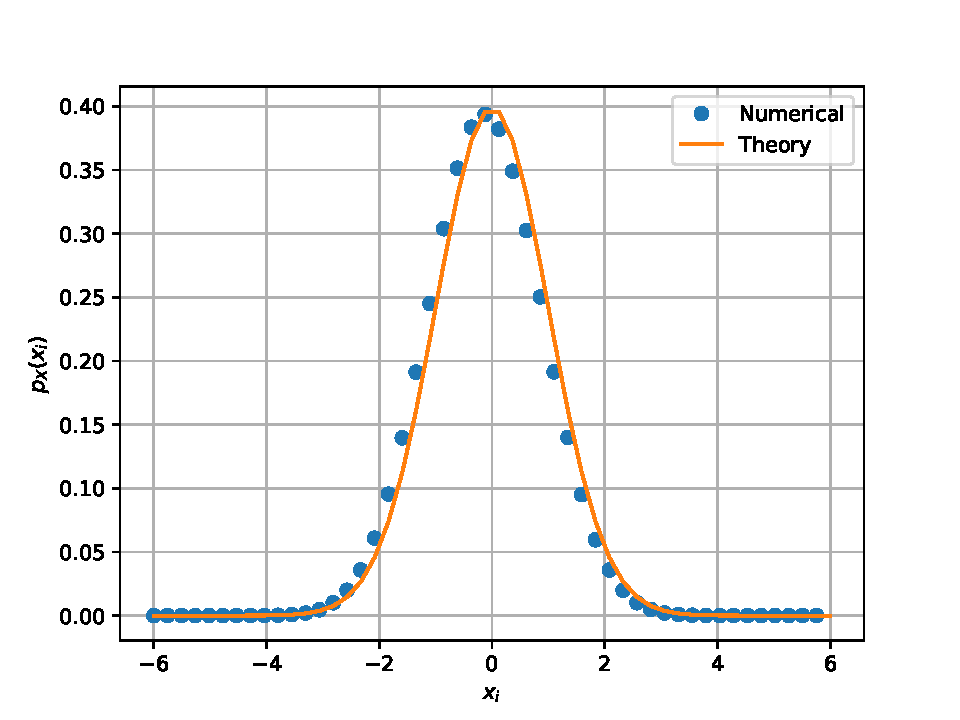
\includegraphics[scale=0.8]{chapter2/figs/gauss_pdf.pdf}
\caption{The PDF of $X$}
\label{fig:gauss_pdf}
\end{figure}

The properties of PDF are
\begin{eqnarray}
	f_X(x) \ge 0 \text{for all} X \in \mathbb{R} \\
	\int_{-\infty}^{\infty} f_X(x) \,dx = 1
\end{eqnarray}

\item Find the mean and variance of $X$ by writing a C program.  \\
\solution The following code prints the mean and variance of $X$
\begin{lstlisting}
	chapter2/codes/mean.c
\end{lstlisting}
The output of the program is
\begin{lstlisting}
Gaussian stats:
Mean: 0.000294
Variance: 0.999561	
\end{lstlisting}
\item Given that 
\begin{align}
p_{X}(x) = \frac{1}{\sqrt{2\pi}}\exp\brak{-\frac{x^2}{2}}, -\infty < x < \infty,
\label{eq:gau_pdf}
\end{align}
repeat the above exercise theoretically.\\
\solution The mean of gievn PDF is given by $E\sbrak{X}$ ,
\begin{flalign}
	E\sbrak{X} = \mu_X &= \int_{-\infty}^{\infty} \frac{1}{\sqrt{2\pi}}\exp\brak{-\frac{x^2}{2}} \,dx&\\
     = \frac{1}{\sqrt{2\pi}} \int_{-\infty}^{\infty} x e^{-\frac{x^2}{2}}dx\\
    &=0 & \\ 
	\mu_X &= 0
\end{flalign}
Variance is given by
\begin{align}
    \sigma^2 =  E\brak X^2 - E^2\brak X 
\end{align}
Substituting $\mu_X$ and the PDF
\begin{flalign}
	 &= \frac{1}{\sqrt{2\pi}} \int_{0}^{\infty} x^2 e^{-\frac{x^2}{2}} dx\\
    &= \frac{2}{\sqrt{2\pi}}\int_{0}^{\infty}\sqrt{2u}e^{-u} du \quad\brak{Let \frac{x^2}{2}= u}\\
    &= \frac{2}{\sqrt{\pi}} \int_{0}^{\infty} e^{-u} u^{\frac{3}{2}-1} du \quad\brak{Let \Gamma\brak{\frac{1}{2}}=\sqrt{\pi}}\\
    &= \frac{2}{\sqrt{\pi}} \Gamma\brak{{\frac{3}{2}}}\\
    &= \frac{1}{\sqrt{\pi}}\Gamma\brak{\frac{1}{2}} \\
    &= 1
\end{flalign}
%
\end{enumerate}


\section{From Uniform to Other}
\begin{enumerate}
%
\item
Generate samples of 
%
\begin{equation}
V = -2\ln\brak{1-U}
\end{equation}
%
and plot its CDF. \\
\solution
\begin{lstlisting}
	chapter2/2_3_cdf.py
\end{lstlisting}
\begin{figure}[H]
\centering
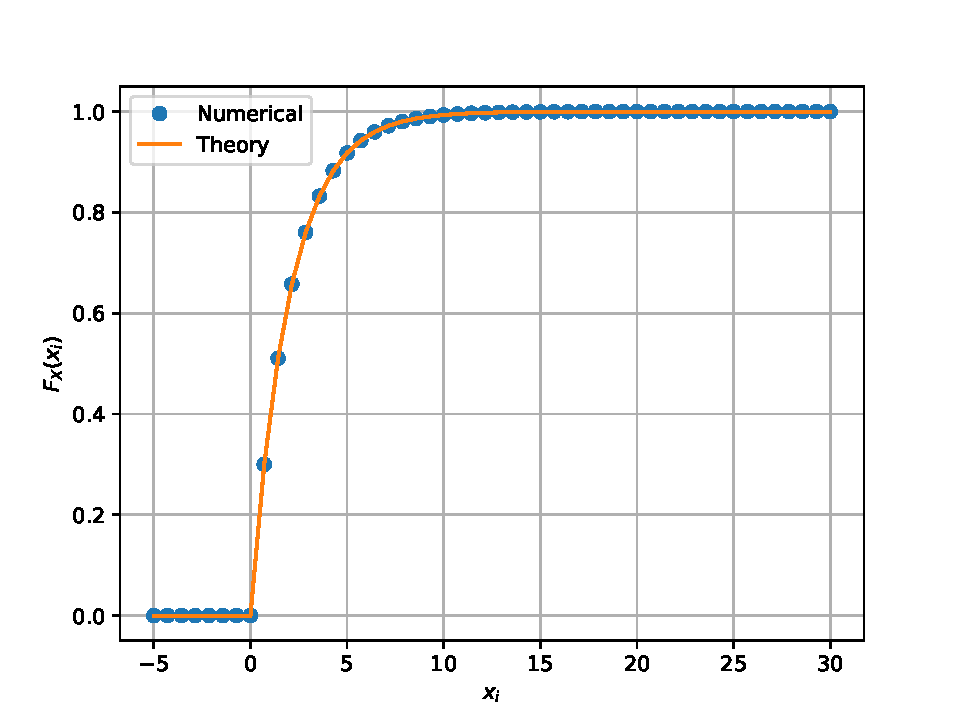
\includegraphics[scale = 0.7]{chapter2/figs/log.pdf}
\caption{The CDF of $V$}
\label{fig:log_uni_cdf}
\end{figure}
\item Find a theoretical expression for $F_V(x)$.
\begin{flalign}
	F_V(x) &= P(V \le x)&\\
	&= P(-2\ln\brak{1-U} \le x)&\\
	&= P(U \le 1 - e^{\frac{-x}{2}})&\\
	&= F_U(1 - e^{\frac{-x}{2}})
	\label{eq:probman_cdf_V_temp}
\end{flalign}
\begin{align}
F_U(x) = 
\begin{cases}
0 &  x < 0 \\
x & 0 \le x \le 1 \\
1 & x > 1
\end{cases}
\end{align}
%
Substituting the above in \eqref{eq:probman_cdf_V_temp},
%
\begin{align}
F_U\brak{1- e^{-\frac{x}{2}}} =
\begin{cases}
0 &  1- e^{-\frac{x}{2}} < 0 \\
1- e^{-\frac{x}{2}} & 0 \le 1- e^{-\frac{x}{2}} \le 1 \\
1 & 1- e^{-\frac{x}{2}} > 1
\end{cases}
\end{align}
After some algebra, the above conditions yield
\begin{align}
F_V(x) = 
\begin{cases}
0 & x < 0 \\
1- e^{-\frac{x}{2}} & x \ge 0
\end{cases}
\label{eq:probman_V_cdf_anal}
\end{align}
\end{enumerate}


\section{Triangular Distribution}
%
\begin{enumerate}
\item Generate 
	\begin{align}
		T = U_1+U_2
	\end{align}\\
\solution Download the following files and execute the  C program.
\begin{lstlisting}
chapter2/codes/tri.c
\end{lstlisting}
\item Find the CDF of $T$.\\
\solution 
\begin{lstlisting}
	chapter2/codes/tcdf.py
\end{lstlisting}
\begin{figure}[H]
\centering
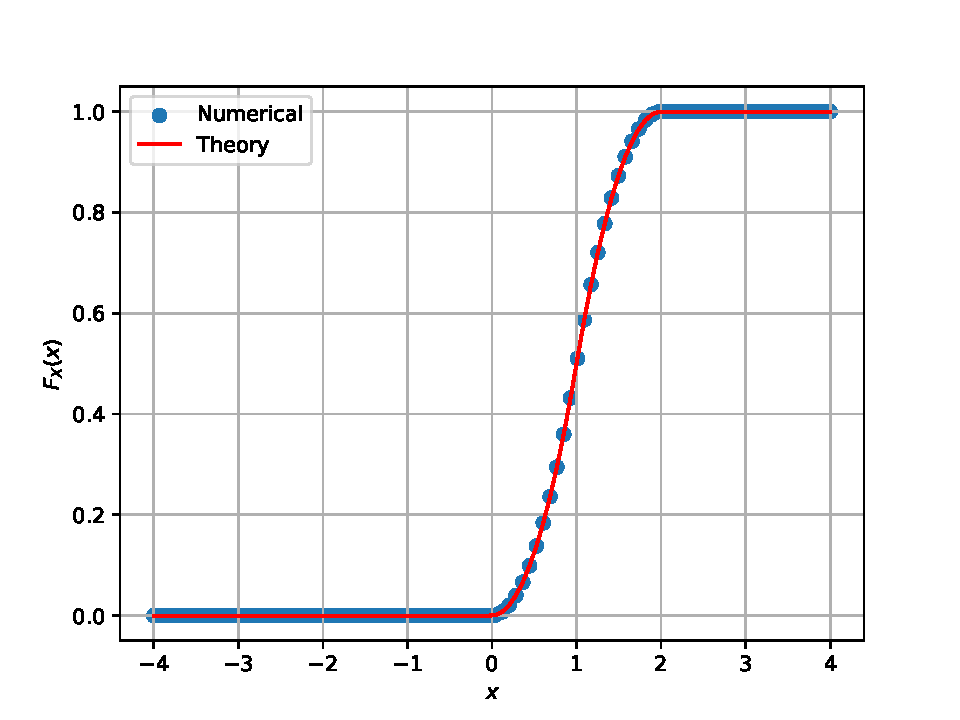
\includegraphics[scale=0.8]{chapter2/figs/triangle_cdf.pdf}
\caption{The CDF of $T$}
\label{fig:tri_cdf}
\end{figure}
\item Find the PDF of $T$.\\

\begin{lstlisting}
chapter2/codes/tdpf.py
\end{lstlisting}
\begin{figure}[H]
\centering
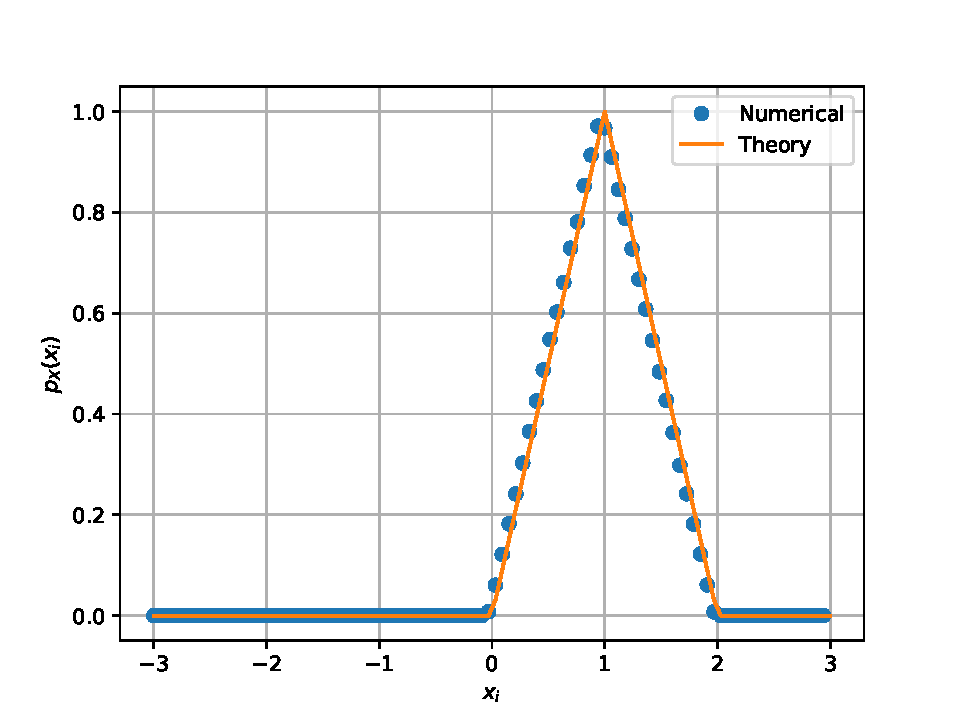
\includegraphics[scale=0.8]{chapter2/figs/triangle_pdf.pdf}
\caption{The PDF of $T$}
\label{fig:tri_pdf}
\end{figure}
\item Find the theoretical expressions for the PDF and CDF of $T$.\\
\solution 

CDF $F_U(x)$ is
\begin{align}
F_{T}(x) &= 
\begin{cases}
0 & x \leq a \\
\frac{(x-a)^2}{(b-a)(c-a)} & a < x \leq c \\
1-\frac{(b-x)^2}{(b-a)(c-a)} & c < x \leq b\\
1 & x > b
\end{cases}
\end{align}
PDF $p_T(x)$
\begin{align}
p_{T}(x) = \frac{d}{dx}F_{T}(x)
\end{align}
\begin{align}
p_{T}(x) &= 
\begin{cases}
0 & x \leq a \\
\frac{2(x-a)}{(b-a)(c-a)} & a < x \leq c \\
\frac{2(b-x)}{(b-a)(c-a)} & c < x \leq b\\
0 & x > b
\end{cases}
\end{align}

\item Verify your results through a plot. \\
\solution Refer the \figref{fig:tri_cdf} and \figref{fig:tri_pdf}
\end{enumerate}
